\documentclass[12pt]{article}
\usepackage[margin=0.75in]{geometry}
\usepackage{amssymb}
\usepackage{amsmath}

\ifx\pdfoutput\undefined
     \usepackage[dvips]{graphicx}
\else
     \usepackage[pdftex]{graphicx}
     \pdfcompresslevel 9
\fi

\usepackage{parskip}
%%\setlength{\parindent}{1cm}

\raggedright

\begin{document}

\begin{center}

{\LARGE The Virtual Machine for Quadruples}
\newline
{\large A simple machine architecture for testing compilers}
\newline
{\large Version 2.0 September, 2002}
\newline
{\large R. L. Zarling}
\newline
\end{center}

\section*{{\large INTRODUCTION}}

The Virtual Machine for Quadruples, {\em vmq}, implements a small but usable set of operations
commonly found in real hardware architectures using an easily managed, ASCII based, ``object'' format.
This combines portability with the ability to manually examine and even modify ``object'' programs with
a simple text editor. Program trace and memory dump functions are included to aid debugging. It supports
a limited set of data types: 16-bit integers, 32-bit floats, 16-bit pointers and character strings. A system stack
is used for subroutine linkage and local data storage.

\section*{File Format}
Vmq ``object'' files are line-based ASCII files organized into two distinct sections: the global data section
followed by the instruction section. The global data section normally contains storage for all of the constants
used in the program, as well as globally accessible variables. The instruction section contains executable
instructions in the form of ``quadruples'':  an ``operation code'' followed by up to three operands. Lines may
not begin with optional white space, and comment lines are not permitted (although any line, including a
no-op instruction, may have comments at the end of the active information).

\section*{Data Types}
Supported data types are 16-bit decimal integers, single-precision decimal floats (expressed with a decimal point),
character strings in quotation marks (") whose length is the string length plus one (for a terminating '0'), and
2-byte addresses. Integers and addresses must be aligned on an even storage boundary; floats must be aligned
on a four-byte boundary. Integer, float and string constants may be initialized by a line in the quadfile Data Section
which begins with a decimal address and then gives the constant value to be stored there. As with the rest of the
quadfile, anything on the line following the data value is a comment.
\newpage
\section*{Virtual Machine Operations}
     Each line of the code section represents one instruction. The following table summarizes the available operations.
Note that Operation Codes are all a single character; in general, lower-case codes represent integer operations
and upper-case represents float operations. Thus, for example, `a' is integer addition, while `A' is floating point addition.
Operands may be of several types: addresses, interpreted as either an r-value or an l-value and specified in one of three
addressing modes; labels which specify the location of a quadruple assuming the first quadruple in the code section
is number 0; or integer constants, which are simply signed 16-bit integers. All numeric quantities are always given in base 10.

\begin{tabular}{ | l r | l | l | l | }
    \hline
     Operation & & Operand 1 & Operand 2 & Operand 3 \\ \hline
     Add: `a' or `A'  & o3 = o1 + o2 & r-val: int or float &  r-val: int or float  &  l-val: int or float \\
     Subtract: `s' or `S'  & o3 = o1 - o2 & r-val: int or float &  r-val: int or float  &  l-val: int or float \\
     Multiply: `m' or `M'  & o3 = o1 * o2 & r-val: int or float &  r-val: int or float  &  l-val: int or float \\
     Divide: `d' or `D'  & o3 = o1 / o2 & r-val: int or float &  r-val: int or float  &  l-val: int or float \\
     Residue: `r'  & o3 = o1 \% o2 & r-val: int or float &  r-val: int or float  &  l-val: int or float \\
     Bitwise OR: `$|$'  & o3 = o1 $|$ o2 & r-val: int or float &  r-val: int or float  &  l-val: int or float \\
     Bitwise AND: `\&'  & o3 = o1 \& o2 & r-val: int or float &  r-val: int or float  &  l-val: int or float \\
     Jump if $<$: `l' or `L'  & o1 $<$ o2? goto o3 & r-val: int or float &  r-val: int or float  &  Label (quad num) \\
     Jump if $>$: `g' or `G'  & o1 $>$ o2? goto o3 & r-val: int or float &  r-val: int or float  & Label (quad num) \\
     Jump if =: `e' or `E'  & o1 = o2? goto o3 & r-val: int or float &  r-val: int or float  &  Label (quad num) \\
     \hline
    Identity: `i' or `I'  & o2 = o1 & r-val: int or float &  l-val: int or float  &   \\
    Byte copy: `='  & o2 = o1 & r-val: char &  l-val: char  &   \\
    Float: 'F'  & o2 = float(o1) & r-val: int &  l-val: float  & {\large \ \ \ \ N/A} \\
    Int: `f'  & o2 = int(o1) & r-val: float &  l-val: int & \\
    Bitwise NOT: `$\sim$'  & o2 = $\sim$ o1 & r-val: int &  l-val: int &  \\
    Negate: `n' or `N'  & o2 = - o1 & r-val: int or float &  l-val: int or float  & \\
    \hline
    Call function: `c' & o1 = o2() & l-val: integer or &  Label & \\
      &   & \ \ \ \ float or 0 &\ \ \ (quad number)   & {\large \ \ \ \ N/A} \\
    Initialize Runtime & o1 \ \ o2 & Label: main entry& int constant:  & \\
       \ \ \ \ Environment: '\$' &  &  \ \ \ \ address & \ \ \ size of globals & \\
    \hline
    Uncond. jump: 'j' & goto o1 & Label: destination & & \\
    Push: 'p' or 'P' & push (o1) & a function param. & & \\
    Pop n bytes: '$\wedge$' & pop(o1)& int constant:  n &{\large \ \ \ \ N/A} &{\large \ \ \ \ N/A} \\
    & & \ \ \ bytes to pop & & \\
    Create stack fr.: '\#' & link-o1& int constant: & & \\
       &  & \ \ \ size of locals & & \\
     \hline
     Return from func: '/' & return & & & \\
     Halt execution: 'h' & halt & {\large \ \ \ \ N/A} & {\large \ \ \ \ N/A} & {\large \ \ \ \ N/A} \\
     No operation: ';' & noop & & & \\
     \hline
  \end{tabular}
  \newpage
\section*{R-Values and L-Values}
     The term ``r-value'' means an operand that will be evaluated and used in a calculation, while ``l-value'' is an
operand that will be evaluated to an address where a result can be stored. Thus, r-values can be given in any
of the three addressing modes: indirect, direct, or immediate, while l-values must be either indirect or direct.

Direct addressing mode means that the address represents the place in memory where the operand is to be
placed (l-value) or retrieved from (r-value). You specify direct addressing by simply giving the address with no
mode modifiers.

Indirect addressing mode means the operand points to a memory address where the actual effective address
may be found. You specify indirect mode by preceding the address with an ``at'' sign (@).

Immediate addressing mode means the address in the instruction is the data to be worked with. You specify
immediate mode by preceding an address with a sharp sign (\#). Immediate mode cannot be used for l-values.
For floating point operands, the immediate operand must contain a decimal point.

\section*{Base-Relative and Absolute Addressing}
A local (stack-based) address needs to be interpreted as a base-relative offset; that is, it must be added to the base of the current stack frame to find the actual memory location. You may specify such an offset by preceding the address with a slash (/). Since the processor stack grows downward, positive offsets point into the previous activation record and may be used to address parameters. Negative offsets address local variables in the current stack frame. See the section Activation Records below.

You may also specify an absolute memory address if you just supply the address with no `/' modifier. This would ordinarily be used to access constants or global variables in the global data area.
\newpage
\section*{Activation Records and the System Stack}
     Functions use activation records to access parameters, and for storage for a return value, return address, dynamic
     link pointer, and local storage. Activation records are allocated on the system stack, so they are also sometimes 
     called stack frames. They are organized as shown below. Everything on the stack must always be aligned to an even
     address. Use a `p' (or `P') quad to push parameters onto the stack. You may push addresses (``p \#...'')
     or values, depending on the parameter passing method. The `c', `\#', `/' and `$\wedge$' also manipulate the stack.
     
     Note that parameters are pushed in reverse order, so that parameter \#1 is always at offset +6 from the base of the
     activation record. Parameters that the user pushes on the stack are not removed automatically by the system.
     The user may use a `$\wedge$' quad to remove these after the called function returns, or, at the cost of ``wasting'' a bit of
     stack space, they may be simply left on the stack since the stack will be properly reset to the previous
     stack frame when the current function returns.
     \vspace{1.5cm}
      \centerline{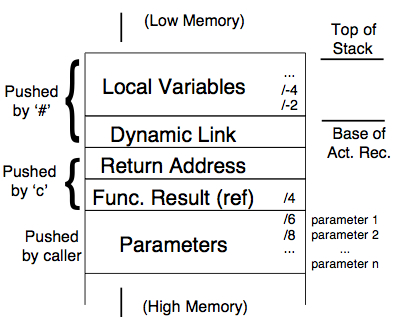
\includegraphics[width = 4.5in]{VMQ-stack-frame}}
     
     
%(Low Memory)
%Top of Stack
%Base of Act. Rec.
%parameter 1 parameter 2 ... parameter n
%?... Local Variables /-4 /-2
%?Dynamic Link
%?Return Address
%?Func. Result (ref) /4
%?/6
%/8 Parameters ...
%Pushed by `\#'
%Pushed by `c'
%Pushed by caller
%?????(High Memory)

The function result address is pushed onto the stack when the function is called (`c' quad). For a function that returns a value, this must always point to a memory location where the return value is to be stored. To return a value, the function should store the value indirectly through this pointer, which is always at offset +4 from the stack base.

You will ordinarily not deal directly with the dynamic link; it is used to locate and re-install the previous activation record when a function return quad (`/') is executed. The dynamic link, return address, and function result reference are popped from the stack automatically when `/' is executed.
The architecture does not have a static chain, although the user could manage his/her own static chain using an emulated static link register in memory and local address -2 (say) for links.

\section*{Notes About the Instruction Set}
\begin{enumerate}
     \item There are only three conditional branch instructions, but that is enough, since you can test,
          for instance, if x is ``not-less-than'' y instead of testing if x is ``greater-than-or-equal-to'' y.
          The conditional branches interpret their operands as signed quantities -- there is no way to reliably
          compare unsigned integers. This is not, however, a problem for comparing memory or quadruple
          addresses, since both are limited to 15 bits.
     \item The `\$' quad must be quadruple number 0, and cannot appear anywhere else in the quad list.
          It will be executed once at the beginning of the run, and must not be executed again.
     \item Every function, including main(), must begin with a `\#' quad to establish a stack frame.
     \item The function-call quad, `c', requires an l-value address into which the function's result will be placed.
          If the function does not return a value, this may be 0. In any event, however, this address will be pushed
          onto the stack as a kind of zeroth parameter. See Activation Records,  below.
     \item Virtual system I/O functions are located at negative ``quad addresses''.  A function at quad number -1 reads
          an integer, number -2 reads a float, and -3 reads a line of characters from cin.
          Quad number -9 prints an integer, number -10 prints a float, and number -11 prints a string to cout.
          All of these require a single parameter to be pushed before the call, the location to be read into or printed from.
          None of them ``returns'' anything.
\end{enumerate}

\section*{Diagnostics}
     Diagnostic requests may appear before any opcode, with no intervening white space.. You may
     use x (begin execution trace), X (end execution trace), or @ (dump current contents of data memory).
     If more than one is given on a single line, they must be in the order x X @. A compiler would ordinarily
     not produce these; you would add them manually during debugging using an editor.
     
     In the diagnostic output, addresses and memory contents are represented in hexadecimal out of respect
     for tradition. Calculated results are shown in both hexadecimal and decimal for convenience. In the dump
     of the stack area, values on the dynamic chain are represented with an underscore character in the middle;
     e.g. 7e\_a2.
     
\section*{Limitations}
     The emulated data memory is 0x7ffc bytes in size. The stack is based at the top of memory and grows downward;
     thus, the stack and the global data area mutually limit each other's maximum size. There cannot be more than 32767
     quadruples in a program; these however are stored in an area that does not overlap data memory.
     
\section*{Sample Programs}
The following GCD program shows one possible set of quads which would implement the sample program shown. The
comments at the ends of the quads are for clarification only; they would not necessarily appear in the actual quad file.
\begin{verbatim}
     000 0                       ;constant 0 at static address 0
     2 "\n"                       ;x & y are at 4 & 6, not initialized
     8 "Enter two integers: "
     29 "The GCD is "
     $ 13 40                    ;Start code section, X & Y are in 4 and 6
     # 4                           ;enter gcd(), a=@/6, b=@/8, tmp0=/-2, tmp2=/-4
     e @/8 0 4                ;if b == 0, goto 4 goto 6
     j 6                            ;if <>0, 
     i @/6 @/4                ;gcd = a 
     j 12                          ;goto return
     r @/6 @/8 /-2          ;form tmp0 = a mod b
     p #/-2                       ;set second parameter = tmp0
     p /8                          ;set first parameter = b
     c #/-4 1                    ;call gcd recursively; result to tmp2
     ^ 4                           ;pop parameters ;store return value
     i /-4 @/4
     /                               ;return from subroutine
     # 2                           ;enter main, 2 bytes of local storage for tmp0=
     p #8                         ;set up string parameter
     c 0 -11                     ;output string
     ^ 2
     p #4                         ; parameter for Read
     c 0 -1                       ;read integer to g4 (x)
     ^ 2
     p #6                         ;parameter for Read
     c 0 -1                       ;read integer to g6 (y)
     ^ 2
     p #29                       ;message as parameter
     c 0 -11                     ;write string
     ^ 2
     p #6                         ;set second parameter = y
     p #4                         ;set first parameter = x
     c #/-2 1                    ;call gcd result to tmp0
     ^ 4
     p #/-2                       ;set parameter for write = tmp0
     c 0 -9                        ;write integer
     ^2
     p #2                          ;string address
     c 0 -11                      ;write string
     ^2
     h
\end{verbatim}
\begin{verbatim}
     // Sample program for C++ subset
     // Computes the GCD of two integers
     
     
     /* include statements are needed for real C++,
         but are simply considered comments in our subset
     */
     #include <iostream>

     int x,y;    //The two values whose GCD is to be computed
     
     
                // In the subset, a and b are passed by reference, but in
                //  real C++, they are passed by value. It doesn't matter
                //   in this program.
           
     int gcd(int a,int b) {
          if ( b == 0 ) return a;
          else return gcd ( b, a % b );
     }

     int main() {
          cout << "Enter two integers: ";
          cin >> x >> y; cout << "The GCD is" << gcd(x,y) << endl;
     }

\end{verbatim}
\newpage
Subscripting Example

The following translates a[5] = 42, assuming a is stored beginning at address 6.
\begin{verbatim}
     000 5              ;array subscript to use
     002 2              ;element size in bytes
     004 42            ;value to be stored
     006 0              ;array start at this address (only 1st element initialized
     $ 1 20             ;20 bytes of global storage
     # 6                  ;6 bytes of local storage (more than really needed)
     xm 0 2 /-2       ;tmp0 = (subscript) * (element size)
     a /-2 #6 /-4      ;tmp2 = (tmp0) + (address of array)
     i 4 @/-4           ;store value in address computed above
     X@;                 ;dump memory so we can see what happened
     h
     
     2: x(m, 0x0000, 0x0002, /0xfffe) --> (0x7ff8) = 0x000a ( = 10 )
     3: (a, /0xfffe, \#0x0006, /0xfffc) --> (0x7ff6) = 0x0010 ( = 16 ) 
     4: (i, 0x0004, @/0xfffc) --> (0x0010) = 0x002a ( = 42 )
     
     Global Data Area:
     0x0000 00 05 00 02 00 2a 00 00 ff ff ff 00 ff ff ff 00
     0x0010 00 2a ff 00
     
     Runtime Stack Area:
     0x7ff4 e0 e0 00 10 00 0a 7f_fc
     
     Stack: 0x7ff4->0x7ffa
\end{verbatim}
\newpage

     Floating Point Example
     
\begin{verbatim}
     
     0 3.14159
     4 2.0
     8 "Enter the radius: "
     27 "The circumference is "
     49 "\n"
     $ 1 51
     #8
     p #8
     c 0 -11
     ^ 2
     p #/-4
     c 0 -2
     ^ 2
     M 0 4 /-8
     M /-8 /-4 /-8
     p #27
     c 0 -11 ^ 2
     p #/-8
     c 0 -10
     ^ 2
     p #49
     c 0 -11
     ^ 2
     @h
\end{verbatim}


\end{document}
